\section{Additional Results and Interpretation}
\label{app:results}

\subsection{Structural contrasts and control scope}

This subsection reports the historical Study~1 results.
The FULL analysis fits all group elements, whereas AFS-A
fits generators and evaluates their products on elements
excluded from direct supervision.
Both use held-out templates and the prediction and
consistency metrics defined in \cref{app:metrics}.
These fitted-map diagnostics are distinct from the
same-bank class-risk bounds and spectral-budget comparisons
in Study~2.
Unless stated otherwise, the intervals below are the
recorded 95\% bootstrap percentile ranges.
Their interpretation is fixed-panel resampling sensitivity,
with the dependencies and limitations described in
\cref{app:inference}.

\begin{table}[t]
\caption{
Held-out FULL errors at $q=16$.
Values are descriptive means over six fixed models,
four specified depths, five splits, and six test templates
per split.
Random-orthogonal values additionally average five
technical control seeds, which are not independent
model replications.
Identity relation scores were not evaluated and are
shown as unavailable.
Lower values indicate smaller errors under the
respective metric.
}
\label{tab:structural-main}
\centering
\small
\begin{tabular}{llrr}
\toprule
Group & Estimator & $\Eeq$ & $\Erel$ \\
\midrule
$C_7$ & Joint             & 0.0493 & 0.0135 \\
$C_7$ & Ridge             & 0.0483 & 0.0305 \\
$C_7$ & Identity          & 1.4458 & -- \\
$C_7$ & Random orthogonal & 2.0297 & 1.8712 \\
\midrule
$D_4$ & Joint             & 0.0529 & 0.0097 \\
$D_4$ & Ridge             & 0.0520 & 0.0170 \\
$D_4$ & Identity          & 1.5300 & -- \\
$D_4$ & Random orthogonal & 1.9978 & 1.9671 \\
\bottomrule
\end{tabular}
\end{table}

\begin{table*}[t]
\caption{
AFS-A generator-composed prediction errors for the five
elements excluded from direct fitting, evaluated on
held-out templates at $q=16$.
Direct Ridge fits each evaluated element separately
and therefore receives additional supervision.
It has lower mean error in both domains; this is not
a claim about every individual condition.
The final column reports the paired composed-minus-direct
contrast and its recorded 95\% bootstrap percentile range.
The fixed-panel and overlapping-partition limitations
in \cref{app:inference} apply.
}
\label{tab:generator-transfer}
\centering
\small
\begin{tabular}{lrrl}
\toprule
Group & Composed & Direct & Composed minus direct \\
\midrule
$C_7$ & 0.0744 & 0.0511
      & $0.0233\;[0.0040,\,0.0471]$ \\
$D_4$ & 0.0566 & 0.0500
      & $0.0065\;[0.0043,\,0.0094]$ \\
\bottomrule
\end{tabular}
\end{table*}

\begin{figure}[t]
\centering
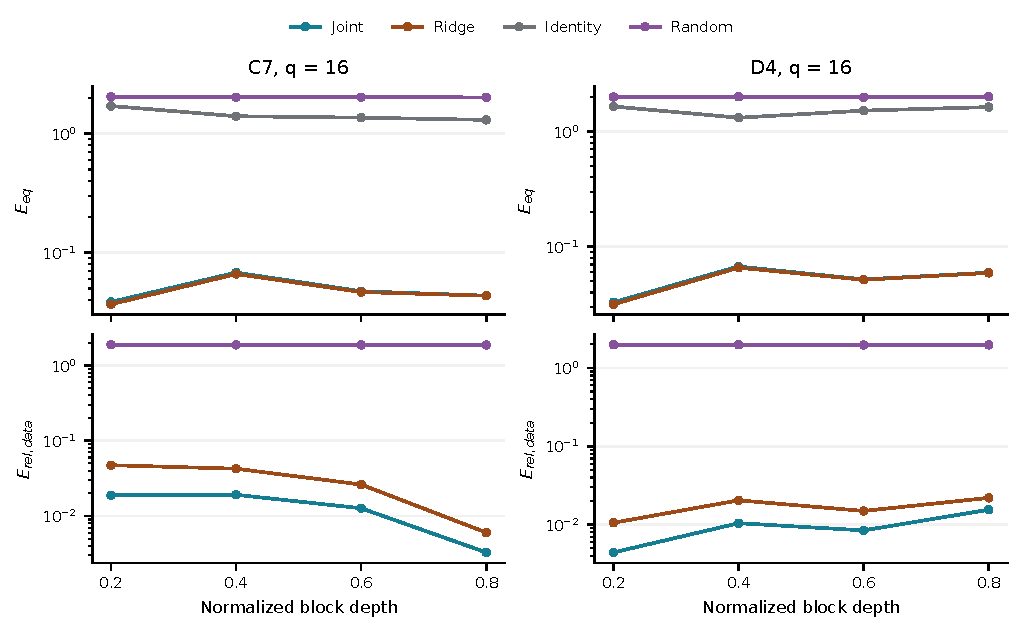
\includegraphics[width=.85\textwidth]
{figures/structural_errors.pdf}
\caption{
Historical FULL prediction and relation diagnostics
across the fixed six-model panel at $q=16$.
Identity relation scores were not evaluated and are
omitted as unavailable, rather than assigned zero.
Joint fitting changes the prediction--consistency tradeoff.
These diagnostics alone do not establish an exact action
or identify a uniquely supported state correspondence.
}
\label{fig:historical-structural}
\end{figure}

\begin{figure}[t]
\centering
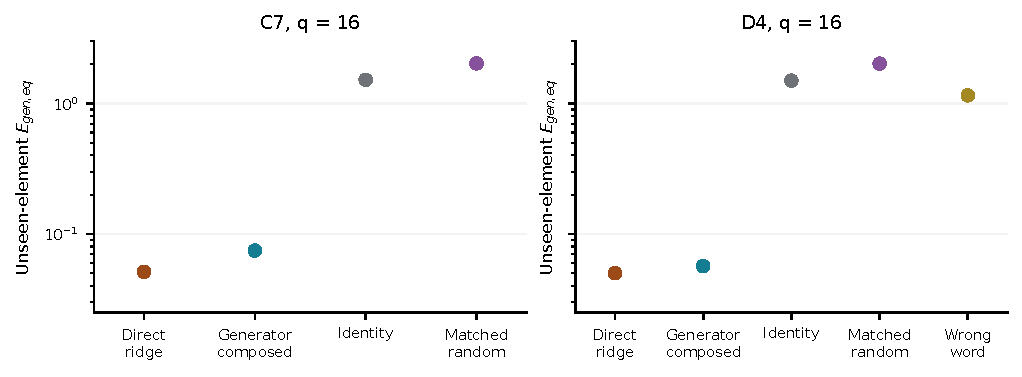
\includegraphics[width=.85\textwidth]
{figures/generator_transfer.pdf}
\caption{
AFS-A generator-composed predictions evaluated against
transformed held-out activations.
Direct element-specific Ridge receives additional
supervision.
The historical label ``Matched random'' denotes products
of randomly sampled orthogonal generator matrices using
the same evaluated words; it does not denote matching
in prediction error.
Identity, random-generator products, and the D4
length-matched wrong words address different alternatives.
}
\label{fig:historical-generator}
\end{figure}

The FULL Joint-minus-Ridge contrasts in the data-space
relation diagnostic $\Erel$ are
$-0.01699$ ($[-0.03405,-0.00318]$) for $C_7$ and
$-0.00728$ ($[-0.01248,-0.00259]$) for $D_4$.
Thus Joint has smaller mean relation defects under
this metric.
These are approximate relations evaluated on activations,
not certificates that the fitted matrices define exact
representations on the ambient coordinate space.
In AFS-A, the D4 correct-minus-wrong-word contrast in
held-out generator-composed prediction error
$E_{\mathrm{gen,eq}}$ is
$-1.097329$ ($[-1.219881,-0.953809]$).
Both words are scored against the same prescribed
held-out targets; this is a prediction contrast,
not a relation-defect contrast.

The FULL paired Joint-minus-random contrasts in $\Eeq$
are $-1.9803$ ($[-2.0041,-1.9549]$) for $C_7$ and
$-1.9449$ ($[-1.9562,-1.9325]$) for $D_4$.
The corresponding Joint-minus-identity contrasts are
$-1.3964$ ($[-1.5882,-1.1982]$) and
$-1.4771$ ($[-1.6692,-1.2628]$).
These panel averages show useful transformation prediction
relative to the untrained controls.
Joint-minus-Ridge prediction contrasts are slightly
positive:
$0.001046$ ($[0.000106,0.002285]$) for $C_7$ and
$0.000864$ ($[0.000149,0.001735]$) for $D_4$.
Joint therefore has slightly higher mean prediction error
than independent Ridge in this comparison.

The paired Joint-minus-Ridge contrasts in the data-space
homomorphism diagnostic $\Ehom$ are
$-0.000884$ ($[-0.002083,-0.000018]$) for $C_7$ and
$-0.000891$ ($[-0.001652,-0.000232]$) for $D_4$.
Together with the relation contrasts, these results
describe a tradeoff between predictive fit and the
consistency terms encouraged by Joint training.
The percentile ranges lie on one side of zero under
the recorded resampling procedure; this does not supply
calibrated population inference or resolve the
identification alternatives in \cref{sec:boundaries}.

\begin{table}[t]
\caption{
Recorded FULL consistency diagnostics at $q=16$.
Each entry pairs a data-space diagnostic with its
operator-space counterpart.
Data defects use squared discrepancies, whereas operator
defects use unsquared relative Frobenius norms.
Their normalizations and relation definitions are
specified in \cref{app:metrics}; in particular, the
$C_7$ relation aggregands differ.
The paired values are therefore not on a common
numerical scale.
Composition diagnostics require both group-element
factors to be nonidentity, but retain pairs whose
product is the identity.
}
\label{tab:full-diagnostics}
\centering
\small
\begin{tabular}{llccc}
\toprule
Group & Estimator
& $\Ehom/\Ehomop$
& $\Erel/\Erelop$
& $\Ecomp/\Ecompop$ \\
\midrule
$C_7$ & Joint
& 0.00842 / 0.05850
& 0.01348 / 0.09612
& 0.01145 / 0.07879 \\
$C_7$ & Ridge
& 0.00930 / 0.06202
& 0.03047 / 0.20903
& 0.01266 / 0.08438 \\
$C_7$ & Random
& 1.45937 / 1.03612
& 1.87118 / 1.45048
& 1.98636 / 1.41027 \\
$D_4$ & Joint
& 0.00366 / 0.10143
& 0.00971 / 0.17124
& 0.00477 / 0.13149 \\
$D_4$ & Ridge
& 0.00455 / 0.11897
& 0.01699 / 0.26283
& 0.00594 / 0.15530 \\
$D_4$ & Random
& 1.52346 / 1.08021
& 1.96710 / 1.39203
& 1.98983 / 1.41088 \\
\bottomrule
\end{tabular}
\end{table}

\begin{table*}[t]
\caption{
Historical correspondence controls and the global
additive-field reference.
AFS-B permutes group-element labels of a fixed fitted
matrix family using a restricted reference that excludes
automorphisms.
Its denominator of 120 is six models times four depths
times five splits, not 120 candidate state-action images.
The observed and reference assignments are not established
as exchangeable, so the percentile comparison is not a
calibrated semantic-null test.
AFS-C reports real-minus-scrambled test prediction error
after refitting on perturbed training pairs and evaluating
against unchanged true targets; negative values favor
the real correspondence.
Brackets are the recorded 95\% bootstrap percentile ranges.
The global additive estimator vanishes analytically
on balanced complete state orbits.
}
\label{tab:diagnostic-controls}
\centering
\small
\begin{tabular}{llp{0.49\textwidth}}
\toprule
Control & Group/metric & Recorded summary \\
\midrule
AFS-B & $C_7$, data homomorphism
& 120/120 below reference 2.5th percentile \\
AFS-B & $C_7$, operator homomorphism
& 120/120 below reference 2.5th percentile \\
AFS-B & $D_4$, data homomorphism
& 120/120 below reference 2.5th percentile \\
AFS-B & $D_4$, operator homomorphism
& 120/120 below reference 2.5th percentile \\
AFS-C & $C_7$, state relabel
& $-0.577\;[-0.664,\,-0.488]$ \\
AFS-C & $C_7$, target scramble
& $-0.596\;[-0.686,\,-0.506]$ \\
AFS-C & $D_4$, state relabel
& $-0.765\;[-0.861,\,-0.662]$ \\
AFS-C & $D_4$, target scramble
& $-0.729\;[-0.824,\,-0.627]$ \\
\midrule
Global additive & Balanced complete orbit
& $\widehat v_g=0$ by permutation cancellation \\
\bottomrule
\end{tabular}
\end{table*}

AFS-B preserves the fitted matrix family while changing
which algebraic element each matrix represents.
It does not enumerate coherent state-action images or
compare their spectral budgets, as the Study~2
registration analysis does.
AFS-C instead changes the training correspondence while
retaining the activation multiset, refits Ridge, and
scores it against the true held-out targets.
In both groups and both AFS-C scramble variants,
the recorded mean test prediction and data-relation
defects increase.
The latter are consistency diagnostics on held-out
activations, not additional measurements of semantic-target
prediction accuracy.

In AFS-C, prediction error and operator norms are not
matched across conditions.
Moreover, the $C_7$ power-consistency and $D_4$ $srs$
terms normalize by condition-specific fitted outputs.
Their deterioration therefore does not isolate an
algebraic effect beyond the change in predictive fit.
Neither AFS-B nor AFS-C shows that a coherently registered
alternative action with comparable learnability
would fail.


\subsection{Rank-matched lexical comparison}

AFS-D compares lexical embeddings with internal
representations using independent Ridge.
Both locations retain training projected rank $q=6$
for $C_7$ and $q=3$ for $D_4$.
This two-model comparison is separate from the FULL
analysis at $q=16$.
The audited input spectra and recorded PCA procedure
support the training-rank match; the historical projected
arrays are unavailable for direct remeasurement
(\cref{app:dimension-rank-audit}).

\begin{table*}[t]
\caption{
Rank-matched lexical and internal comparison using
independent Ridge.
The generator-composed endpoint $E_{\mathrm{gen,eq}}$
uses the five elements excluded from generator fitting.
Both locations use $q=6$ for $C_7$ and $q=3$ for $D_4$;
these are not FULL $q=16$ estimates.
Internal means average four fixed depths.
Repeated embedding observations reuse the same lexical
state vectors.
Equal retained rank does not imply equal retention
of total variance or state-dependent information.
}
\label{tab:lexical-control}
\centering
\small
\begin{tabular}{lllrrr}
\toprule
Group & Model & Location
& $\Eeq$ & $E_{\mathrm{gen,eq}}$ & $\Erel$ \\
\midrule
$C_7$ & Llama 1B & Embedding
& $3.64\!\times\!10^{-6}$
& $5.87\!\times\!10^{-5}$
& $6.37\!\times\!10^{-5}$ \\
$C_7$ & Llama 1B & Internal mean
& 0.132327 & 0.198978 & 0.092076 \\
$C_7$ & Qwen 1.5B & Embedding
& $2.48\!\times\!10^{-6}$
& $4.25\!\times\!10^{-5}$
& $4.72\!\times\!10^{-5}$ \\
$C_7$ & Qwen 1.5B & Internal mean
& 0.171656 & 0.315743 & 0.187296 \\
\midrule
$D_4$ & Llama 1B & Embedding
& $4.97\!\times\!10^{-7}$
& $2.97\!\times\!10^{-6}$
& $3.95\!\times\!10^{-6}$ \\
$D_4$ & Llama 1B & Internal mean
& 0.096634 & 0.133246 & 0.051652 \\
$D_4$ & Qwen 1.5B & Embedding
& $3.02\!\times\!10^{-7}$
& $1.80\!\times\!10^{-6}$
& $2.39\!\times\!10^{-6}$ \\
$D_4$ & Qwen 1.5B & Internal mean
& 0.055191 & 0.059383 & 0.027160 \\
\bottomrule
\end{tabular}
\end{table*}

\begin{figure}[t]
\centering
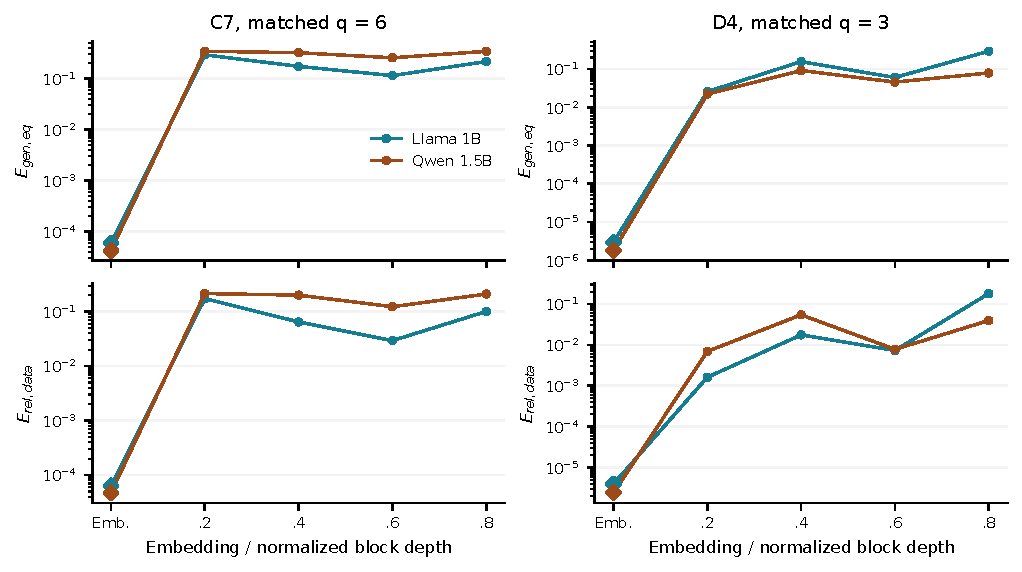
\includegraphics[width=.76\textwidth]
{figures/lexical_internal.pdf}
\caption{
AFS-D lexical and internal errors at matched training
projected rank: $q=6$ for $C_7$ and $q=3$ for $D_4$.
The upper row shows generator-composed prediction error
$E_{\mathrm{gen,eq}}$ on the five excluded elements;
the lower row shows $\Erel$.
The logarithmic axes display descriptive mean errors.
The comparison concerns two models and is separate
from FULL at $q=16$.
Lexical near-exactness is compatible with finite-state
realizability and does not establish a uniquely
supported semantic correspondence.
}
\label{fig:lexical}
\end{figure}

Across the two models and two groups, the
internal-minus-embedding contrasts are positive for
prediction and data-relation error.
Internal representations therefore do not improve these
errors over lexical embeddings under this recorded
rank-matched protocol.
More broadly, all 150 archived metric/depth-summary
intervals have positive lower endpoints.
These comprise 120 depth-specific intervals and
30 intervals for depth-averaged summaries:
two models, six $C_7$ metrics or nine $D_4$ metrics,
and four depths plus their average.
They include metrics not displayed in
\cref{tab:lexical-control}.
They are related summaries of reused observations,
not 150 independent experiments or tests
(\cref{app:inference}).

This comparison does not show that the lexical vectors
encode the uniquely correct semantic action.
For affinely independent lexical state vectors,
retaining the full $(n-1)$-dimensional centered span
permits every state permutation to be realized by a
linear map on that span.
Nor do the observed error differences establish that
internal representations contain less state information.
The result depends on the retained coordinates,
fitting procedure, and evaluation loss.
It does not extend automatically to other models,
dimensions, readout positions, or context constructions.


\subsection{Global additive-field results}

The global additive-field comparator assigns one
source-independent displacement to each group element.
Its recorded direct prediction error is $1.487859$,
compared with $0.050149$ for Ridge and $0.051104$
for Joint.
The additive-minus-Ridge contrast is
$1.437710$ ($[1.400230,1.475673]$), and the
additive-minus-Joint contrast is
$1.436755$ ($[1.399237,1.474462]$).

For these direct-error summaries, the analysis averages
the evaluated actions within each domain and condition,
gives equal weight to model--depth conditions and
domains within each split, and then averages the
five split summaries.
The Ridge and Joint point estimates coincide with
the equal-domain averages of the primary FULL means.
The additive point estimate coincides with the
corresponding identity baseline.
The uncertainty calculations differ:
the additive-field analysis resamples five paired
split-level contrasts, whereas FULL uses the
hierarchy in \cref{app:inference}.

The repeated-composition comparisons use the Ridge
and Joint matrices from FULL, where all elements
were fitted.
They are not additional AFS-A generator-only results.
For $C_7$ powers $r^k$, $k=2,\ldots,6$, the mean
errors are $1.519200$, $0.074443$, and $0.070297$
for additive, Ridge, and Joint, respectively.
For the combined D4 application sequences
$r\to s$, $s\to r$, and $s\to r\to s$,
the corresponding errors are
$1.266128$, $0.049265$, and $0.047450$.
The arrows here specify the order in which the
updates are applied.

The global displacement estimator vanishes for every
group element because the training set contains
complete, balanced state orbits.
For each template, a permutation preserves the sum
of the state vectors, so
\[
 \sum_{i\in S}
 \bigl(h_{g(i),t}-h_{i,t}\bigr)=0.
\]
Averaging these differences over states and templates
therefore gives $\widehat v_g=0$.
The fitted global additive predictor consequently
reduces to identity, and repeated updates remain
identity.
Its failure already occurs for the cyclic task.
The D4 result therefore does not isolate an effect
of noncommutativity, although the commutativity
of translations is an additional limitation of
this edit class.
The result does not rule out source-conditioned
or other additive predictors.

The D4 order-separation diagnostic compares the
outputs of the two application sequences
$r\to s$ and $s\to r$ using
\[
 s(a,b)=
 \frac{\|a-b\|_2^2}
 {\tfrac12\bigl(\|a\|_2^2+\|b\|_2^2\bigr)+10^{-12}}.
\]
Each method uses its own two output vectors in
both the numerator and denominator.
The recorded mean separation is $2.2133$ for the
actual contextual targets, $2.2789$ for Ridge
predictions, and $2.2526$ for Joint predictions.
The additive separation is zero by construction.
These are descriptive separation scores under a
symmetric energy normalization.
They are neither the row-target-normalized loss
$D$ nor prediction accuracies, and they are not
independent confirmatory tests.


\subsection{Behavioral patching}
\label{app:behavior}

The evaluation prompt appends
`` Report the transformed state:''
to a held-out structural prompt.
The source state remains visible.
The particular transformation is supplied through
the selected activation intervention, rather than
through an explicit textual instruction naming $g$.
This setup tests the downstream effects of an
externally chosen edit; it does not establish
which transformation the unpatched model would
compute on its own.

The learned edits use the FULL Joint matrices,
trained with supervision for all group elements.
Let $M_w$ denote the matrix applied in an intervention,
which may be a directly fitted matrix or a product
specified by a word $w$.
This distinction matters when a composed word,
a direct reference, and a wrong-word control
are compared.
Let $\bar h$ be the mean hidden vector over the
selected state span in the evaluation prompt,
let $U_{\mathrm{PCA}}$ be the structural training-only
PCA basis, and define
\[
 z=(\bar h-\hat\mu)U_{\mathrm{PCA}}.
\]
The replacement vector is
\[
 h'
 =
 \bar h-zU_{\mathrm{PCA}}^\top
 +(zM_w)U_{\mathrm{PCA}}^\top.
\]
The forward hook writes this vector to every token
position overlapping the state string at the selected
transformer block output, then recomputes the
remaining network.

The historical control called ``Identity'' uses the
original unpatched output.
It is not an identity-matrix patch.
If the state span contains multiple tokens with
vectors $h_j$, the intervention satisfies
\[
 h'-h_j
 =
 (zM_w-z)U_{\mathrm{PCA}}^\top
 - (h_j-\bar h).
\]
Thus only the change to the span mean is restricted
to the retained PCA subspace.
Writing the same vector to all selected positions
also removes token-specific deviations from the mean,
which need not lie in that subspace.
Even setting $M_w=I$ need not reproduce the
unpatched computation.
The historical experiment contains no matched
zero-delta or token-deviation-preserving sham.
The one-token continuation counts reported below
do not establish that the input state spans
contain one token.

The source-conditioned additive comparator is fitted
on structural training prompts in the original
hidden dimension:
\[
 v_{g,i}
 =
 \frac{1}{|\mathcal T_{\mathrm{train}}|}
 \sum_{t\in\mathcal T_{\mathrm{train}}}
 \bigl(h_{g(i),t}-h_{i,t}\bigr),
 \qquad
 h'=\bar h+v_{g,i}.
\]
It uses the known source-state identity and one
displacement per group-element/source-state pair.
It therefore has different information and
parameterization from a source-shared linear map.
The two edit classes are not generally nested:
the additive displacement is conditioned on the
state label, whereas a shared linear map can
respond to contextual variation in its input.
The additive displacement acts in the original
hidden space, while the learned matrix changes
the PCA component of the span mean.
This comparison avoids global orbit-averaging
cancellation, but it is not a parameter-,
information-, or edit-subspace-matched test of
steering optimality.

In the recorded D4 relation rows, the additive
comparator is indexed by the requested target element.
The true word, its direct reference, and the wrong
word therefore receive the same endpoint-conditioned
displacement.
Their equality for this comparator follows from
the construction and does not test additive
composition order.

The target-token score uses the first token of the
context-sensitive continuation `` \{target state\}''.
Target-logit and target-probability changes subtract
the corresponding values from the unpatched prompt.
The margin is the target first-token logit minus
the original-state first-token logit.
Top-1 success requires the vocabulary argmax to
equal the target token.
The implementation records full target-sequence
log probability only for one-token continuations
and omits that metric for multi-token continuations.
All archived evaluated continuations contain one
token.
These top-1 results therefore concern the scored
continuation token, not general multi-token
answer accuracy.

\begin{table*}[t]
\caption{
Behavioral contrasts from externally applied FULL
Joint edits.
The first four rows summarize transformation
interventions: $r^1,\ldots,r^6$ for $C_7$ and
$r,s,r^2,r^3$ for $D_4$.
Cycle and relation diagnostics are evaluated separately.
``Unpatched'' is the baseline called ``Identity''
in the historical outputs.
Additive denotes the training-only source- and
transformation-conditioned comparator, not the
global additive field.
Positive logit or top-1 differences favor the
learned edit; pp denotes percentage points.
Brackets give the recorded 95\% bootstrap percentile
ranges, interpreted as fixed-panel resampling
sensitivity (\cref{app:inference}).
}
\label{tab:causal-main}
\centering
\small
\begin{tabular}{llll}
\toprule
Group & Metric
& \shortstack{Learned minus\\unpatched}
& \shortstack{Learned minus\\additive} \\
\midrule
$C_7$ & Target logit
& $1.129\;[0.791,\,1.400]$
& $-0.105\;[-0.227,\,-0.014]$ \\
$C_7$ & Top-1 (pp)
& $1.743\;[-0.215,\,3.945]$
& $-0.261\;[-1.065,\,0.056]$ \\
$D_4$ & Target logit
& $2.406\;[1.932,\,2.833]$
& $-0.007\;[-0.030,\,0.012]$ \\
$D_4$ & Top-1 (pp)
& $9.019\;[3.186,\,15.339]$
& $-0.043\;[-0.503,\,0.434]$ \\
\midrule
\multicolumn{4}{l}{
$D_4$ correct-minus-wrong final-logit distance:
$-0.0422\;[-0.0543,\,-0.0298]$.
} \\
\bottomrule
\end{tabular}
\end{table*}

\begin{figure}[t]
\centering
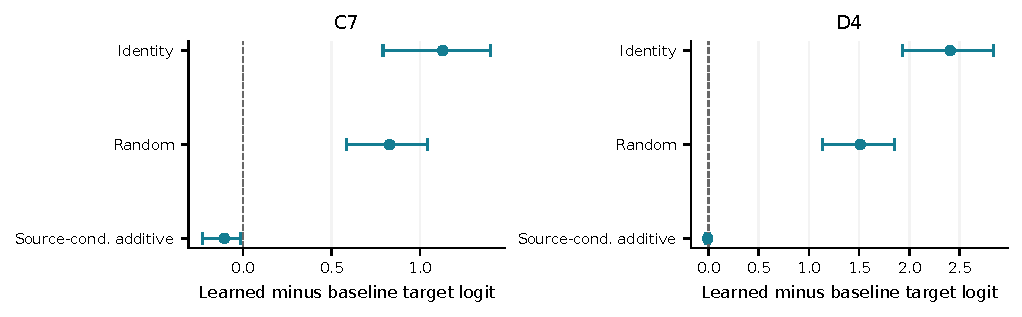
\includegraphics[width=.76\textwidth]
{figures/causal_additive.pdf}
\caption{
Learned-minus-control target-logit contrasts for
transformation interventions.
The historical figure label ``Identity'' denotes
the unpatched baseline.
The other controls use random-generator products
and source-conditioned additive edits.
Negative differences favor the named control
for this outcome.
Bars retain the recorded 95\% bootstrap percentile
ranges.
These downstream effects do not demonstrate
causal necessity of the learned matrix family.
}
\label{fig:causal}
\end{figure}

For $C_7$, powers $r^1,\ldots,r^6$ are transformation
interventions, while $r^7$ is a separate cycle
diagnostic.
For $D_4$, transformation interventions use
$r,s,r^2,r^3$.
The identity-recovery words are $r^4$ and $s^2$,
and the relation diagnostic compares the word
$srs$ with a direct $r^{-1}$ intervention.
The length-matched wrong word is $rsr$.
Although $srs$ and $rsr$ represent different group
elements, they have the same target on two of the
four corners; the wrong-word control does not
change the target for every source state
(\cref{app:faithful-not-free}).

For final next-token logit vectors $L$, the
relation distance is
\[
 d(w,r^{-1})
 =
 \frac{\|L^{(w)}-L^{(r^{-1})}\|_2}
 {\max\bigl(\|L^{(r^{-1})}\|_2,\epsilon\bigr)},
\]
where $\epsilon$ is float64 machine epsilon in
the recorded implementation.
The correct-minus-wrong distance contrast is
$-0.04220$ ($[-0.05426,-0.02981]$).
Both words are compared with the same direct
learned reference.
This is an order-sensitive downstream consistency
diagnostic, not a comparison with a uniquely
identified causal mechanism.

For $C_7$ transformation interventions, the
learned-minus-unpatched target-logit contrast is
$1.129$ ($[0.791,1.400]$), and the
learned-minus-random contrast is
$0.828$ ($[0.585,1.041]$).
The C7 top-1 contrast against the unpatched
baseline has a percentile range spanning zero.
The corresponding D4 top-1 contrast is
$9.019$ percentage points ($[3.186,15.339]$).
The learned-minus-additive target-logit range
lies below zero for $C_7$ and spans zero for
$D_4$.
These observations do not establish a uniform
advantage of the learned edits over the
source-conditioned additive comparator.
A range spanning zero also does not establish
equivalence.

The results show that these interventions can
affect the scored outputs, while leaving substantial
ambiguity about native computation.
The distinction between an editable representation
and the mechanism used by the unpatched model
also matters when interpreting calendar and
group-operation interventions
\citep{engels2025notall,wu2025unified,feucht2026arithmetic}.
Here the transformation is externally selected,
and the intervention and comparator differences
prevent a claim of causal necessity for the
fitted operator family.

\FloatBarrier


\subsection{Cross-model compatibility}

The analysis uses nine fixed model pairs:
all three within-Llama pairs, all three within-Qwen
pairs, and the three size-matched cross-family
pairs, 1B/1.5B, 3B/3B, and 8B/7B.
The operator families are the FULL Joint fits.
For two systems $R_A,R_B$, a row-coordinate
map $T$ is assessed through
\[
 R_A(g)T \approx T R_B(g).
\]
The implementation writes $T=P^\top$ and stacks
the residuals
\[
 P R_A(g)^\top-R_B(g)^\top P.
\]
The smallest right singular vector minimizes
their summed squared Frobenius norm subject to
$\|P\|_F=1$.
This optimization permits singular or low-rank
maps; it does not require an invertible
change of coordinates.

Evaluation reports the normalized score
\[
 \frac{
 \mathbb E_g
 \|P R_A(g)^\top-R_B(g)^\top P\|_F^2
 }{
 \mathbb E_g\|R_B(g)^\top P\|_F^2+10^{-12}
 }.
\]
The singular-vector solution minimizes the
unnormalized numerator, not this ratio.
A small score can therefore indicate compatibility
on a low-rank common subspace without establishing
equivalence of the full representations.

The comparators are an orthogonal Procrustes map,
random orthogonal maps, and shuffled group labels.
Procrustes is fitted to registered test-template
activation pairs after centering their retained
16-dimensional PCA coordinates.
It optimizes activation reconstruction.
The intertwiner instead fits the operators using
the same group elements on which its residual
is reported.
The comparison is therefore descriptive and
uses two fitting criteria on different objects;
it is not predictive transport to unseen paired
activations or held-out elements.
The shuffled-label control retains the map fitted
under the true labels rather than refitting it
after shuffling.
It tests the sensitivity of that map to the
assignment of group labels, not the best achievable
fit under each alternative assignment.
Some shuffled-label comparisons can also be
near-degenerate.

The fitted-minus-Procrustes normalized residual
differences range approximately from $-0.168$
to $-0.065$ across the four domain-by-pair-type
strata: $C_7$ or $D_4$, each with within-family
or cross-family pairs.
All four recorded percentile ranges lie below
zero.
These are stratum-level contrasts, not a claim
that every model--depth--split observation favors
the fitted map.
They show that the fitted commutation maps have
lower mean reported residuals than the selected
geometry alignments in these comparisons.
They do not establish invertible cross-model
representation equivalence.

Linear CKA is computed on the full hidden readouts
before PCA, whereas the commutation score uses
the fitted 16-dimensional operator systems.
The recorded Spearman association between CKA
and negative fitted commutation error is
$-0.014$, with percentile range
$[-0.300,0.287]$.
The pooled calculation contains 360 observations:
nine model pairs, two domains, four depths,
and five splits.
These are not 360 independent samples.
The 5,000 bootstrap draws resample model pair,
then depth, then split, keeping the two domains
together within each terminal block.
The range describes sensitivity under that
historical procedure and does not establish
statistical independence of geometry and
operator compatibility.

Unlike implementation-family comparisons based
on causal abstractions and Congruity
\citep{sun2026tracking}, this analysis neither
samples behavior-preserving implementations nor
estimates an abstraction-dependent distance
between them.
Its scope is compatibility of the fitted
operator systems under the stated map classes
and evaluation criteria.


\subsection{Completed controls and remaining identification scope}

Study~2 provides state-centroid, residual, and
input-only field comparisons under its own
sampling and normalization contract.
Completed extensions include compact nonlinear
predictors fitted on the full training data,
coherent alternative registrations, direct
context-difference fitting, and peer-method
adaptations (\cref{app:reproduction}).
These results add evidence under their respective
protocols.
They do not remove information, fitting, or
intervention mismatches in the historical
Study~1 comparisons.

The new-context study evaluates transport to
64 assistant-authored paired families per domain
while retaining the previously seen state
vocabulary (\cref{sec:new-context}).
The original and new comparisons differ in
wording, validation-based regularization selection,
and, for $D_4$, action weighting.
Their contrast therefore does not isolate a
causal effect of new wording.
The new bank extends the evaluated context
construction, but it does not establish
cross-vocabulary generalization or transport
to independently sampled human-authored prose.
The fitting and paired-family resampling
procedures are given in
\cref{app:pending-protocols}.

The within-template centering diagnostic adds a
separate qualification to registration preference
(\cref{app:template-centering-sensitivity}).
Using the saved 16-dimensional Study~2 coordinates,
the prescribed weekday image is uniquely leading
by spectral budget in 7/24 original conditions,
15/24 after centering with the original whitening,
and 18/24 after centering and rewhitening.
The corresponding corner counts are 16/24,
0/24, and 0/24
(\cref{tab:template-centering-main}).
For corners, the loss of the original lead
therefore occurs even when the original
whitening metric is retained.

These are rankings by $s_{16}=C_{16}/16$,
not rankings of the unknown exact-action risks
$L^\star$.
Under fixed whitening, removing the state-invariant
component preserves the nontrivial spectral blocks
but changes their competition for the dimension
budget.
Rewhitening additionally changes the metric.
The fixed-whitening centered score is not
substituted into the unit-second-moment risk
bounds.
The ranking changes neither establish that
exact actions cease to exist nor measure
state variation outside the retained PCA space.
They show that the observed registration
preference depends on the state-invariant
component and the metric used to evaluate
the retained representations.

The remaining identification gaps should be
distinguished from the finite-bank results
already established.
Interpreting the historical fitted consistency
diagnostics as additional evidence of semantic
specificity would require controls matched
more closely in direct prediction error and
operator norms.
This limitation does not invalidate the
same-bank bounds on the cost of exact-action
constraints.
Cross-vocabulary generalization requires new
lexical realizations, while broader context
generalization requires additional independently
constructed language settings.
Native causal use requires counterfactual
evidence in a task the unpatched model performs
competently.
Native confirmation remains blocked despite
the completed secondary peer-method adaptations.
It is not inferred from the present activation
edits.

Future method selection using the already
inspected holdout would be exploratory and
would require fresh evaluation before a
confirmatory interpretation.
A wrong-group comparator must also admit the
claimed action on the state set.
For example, no permutation of four states
has order eight, so $C_8$ cannot act faithfully
on the four corners.
Nonfaithful actions through smaller quotients
remain possible and are not excluded by the
exact-action class.
An impossible faithful comparator is not an
error-matched semantic alternative.
